\section{Evaluation}\label{sec:eval}

We evaluate \sysname{} using a testbed experiments and numerical analysis.  We
consider three questions: $(i)$ Can \sysname{} prevent deadlock?  $(ii)$ Is
\sysname{} scalable for large data center networks?, and $(iii)$ Does \sysname{}
have a performance penalty?

%\begin{figure}
%	\centering
%	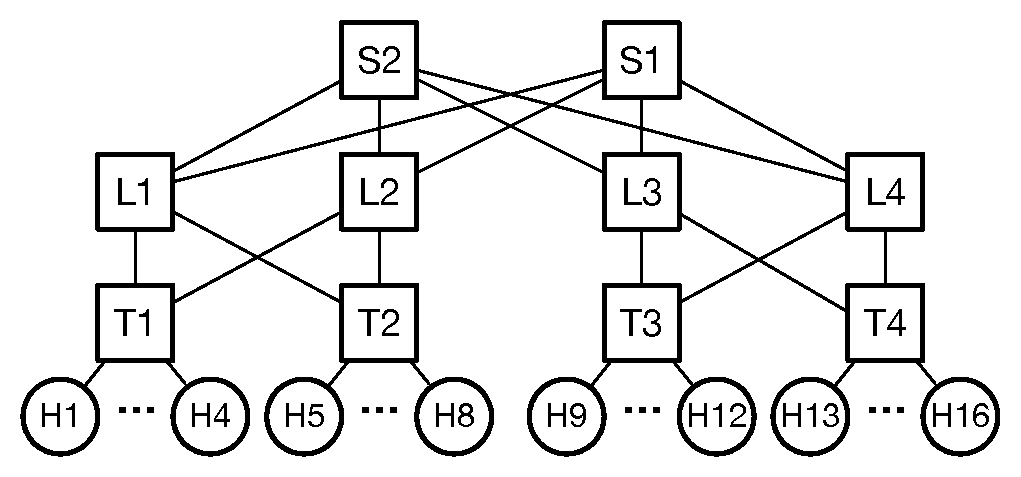
\includegraphics[width=0.45\textwidth] {figs/testbed_topo}
%	\caption{Testbed Topology.}\label{fig:testbed_topo}
%	\vspace{-0.25in}
%\end{figure}

\para{Testbed:} Our testbed (Figure~\ref{fig:basic_clos}) consists of a Clos
network with 10 Arista 7050 (32x40Gb) switches and 16 servers with Mellanox 40Gb
ConnectX-3 Pro NICs.  

\subsection{Deadlock prevention}\label{subsec:exp_validation}

\begin{figure}[t]
	%\vspace{-0.1in}
	\centering
	
	\subfloat[short for lof][Without \sysname] {
		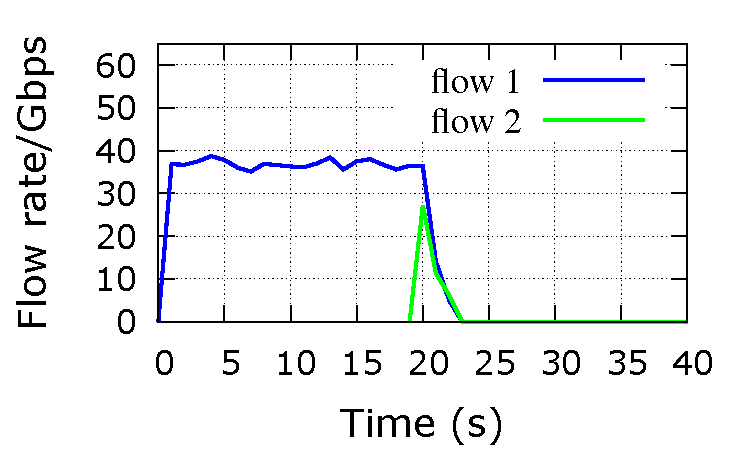
\includegraphics[width=0.25\textwidth] {figs/validation_nonloopcase_flowrate_notagger}
	}
	\subfloat[short for lof][With \sysname]{
		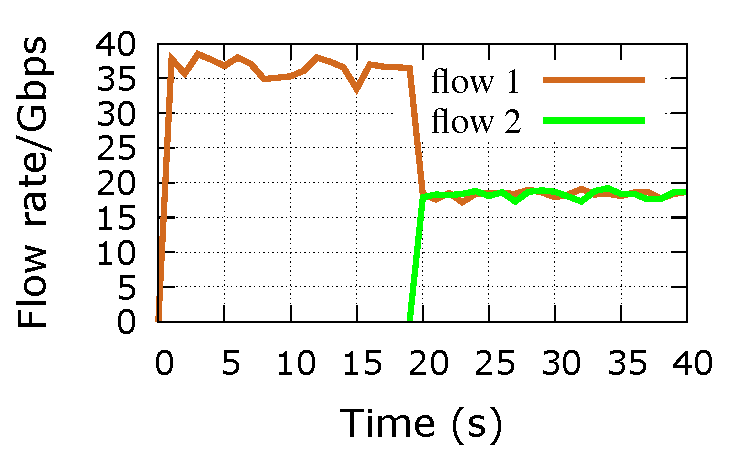
\includegraphics[width=0.25\textwidth] {figs/validation_nonloopcase_flowrate_tagger}
	}
	
	\caption{Clos deadlock due to 1-bounce paths}\label{fig:exp_validation_nonloop}
	\vspace{-0.15in}
\end{figure}

\begin{figure}[t]
	%\vspace{-0.1in}
	\centering
	
	\subfloat[short for lof][Scenario] {
		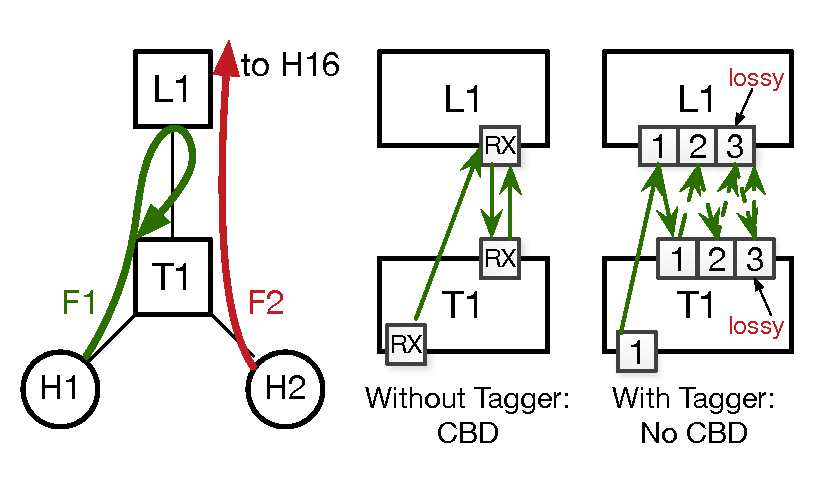
\includegraphics[width=0.4\textwidth] {figs/validation_loopcase_scenario}
	}

\vspace{-0.25in}

	\subfloat[short for lof][Rate of flow 2]{
		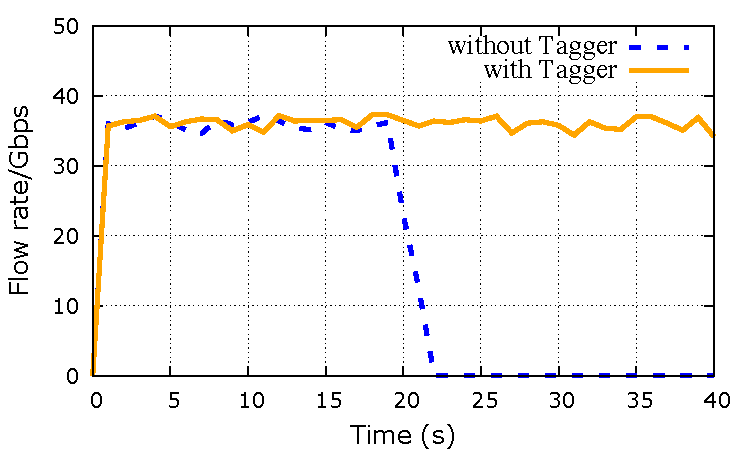
\includegraphics[width=0.4\textwidth] {figs/validation_loopcase_flowrate}
	}
	
	\caption{Deadlock due to routing loop}\label{fig:exp_validation_loop}
	
\end{figure}

\begin{figure}[t]
	%\vspace{-0.1in}
	\centering
	
	\subfloat[short for lof][4-to-1 shuffle with \sysname] {
		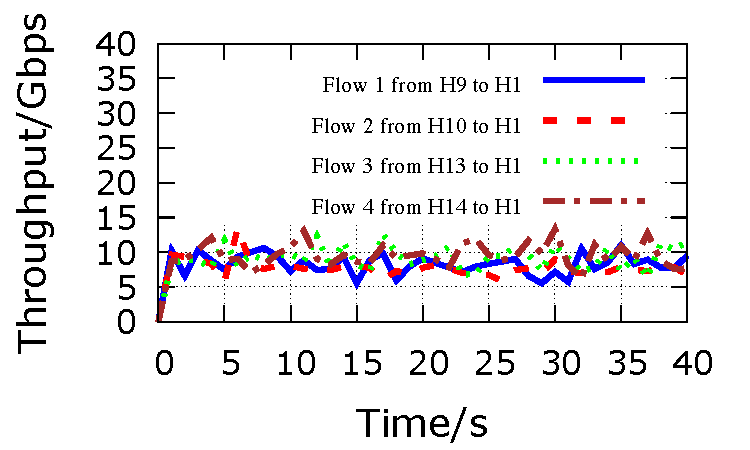
\includegraphics[width=0.25\textwidth] {figs/validation_pp_manytoone_tagger}
	}
	\subfloat[short for lof][4-to-1 shuffle without \sysname]{
		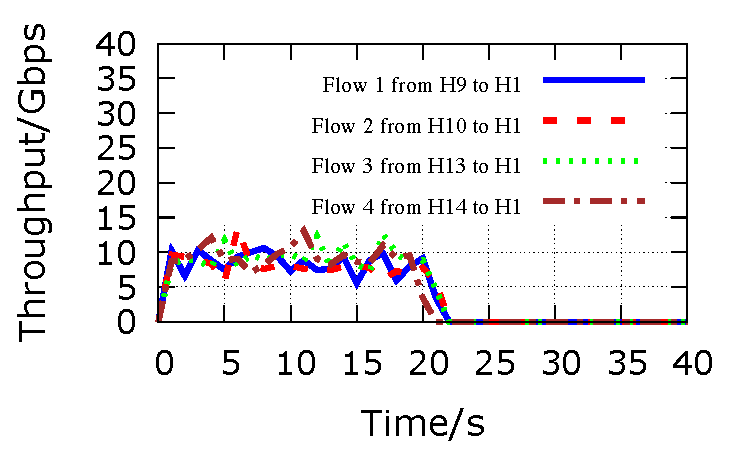
\includegraphics[width=0.25\textwidth] {figs/validation_pp_manytoone_notagger}
	}

	\subfloat[short for lof][1-to-4 shuffle with \sysname] {
	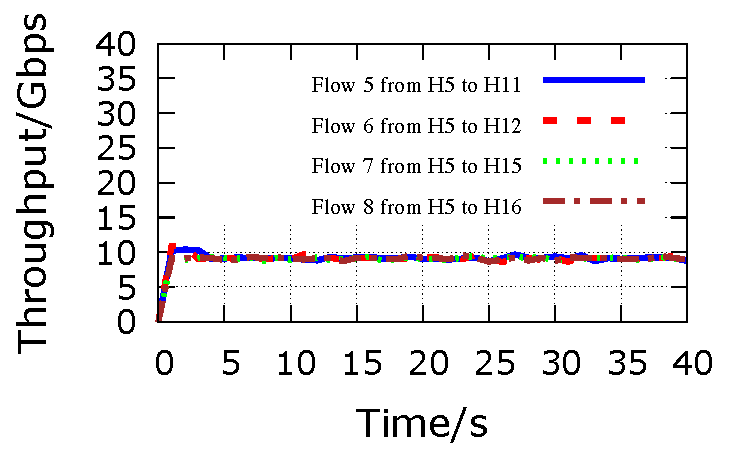
\includegraphics[width=0.25\textwidth] {figs/validation_pp_onetomany_tagger}
}
\subfloat[short for lof][1-to-4 shuffle without \sysname]{
	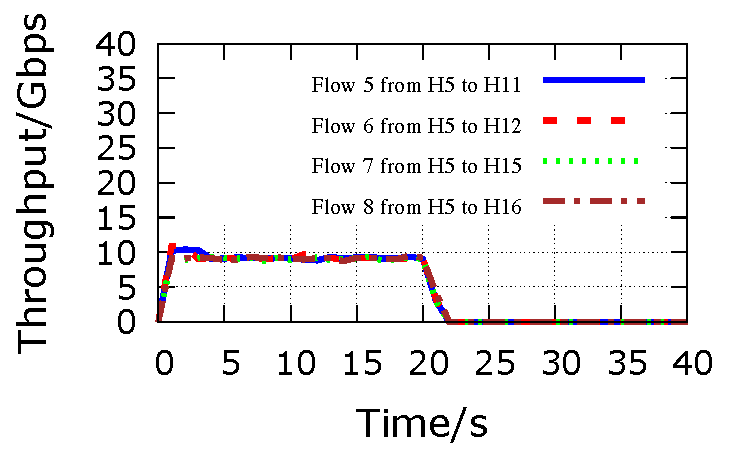
\includegraphics[width=0.25\textwidth] {figs/validation_pp_onetomany_notagger}
}
	
	\caption{PFC PAUSE propagation due to deadlock
	 }\label{fig:exp_validation_propagation}
	
\end{figure}


We have already {\em proved} that \sysname{} prevents deadlock. Thus,
experiments in this section are primarily illustrative. We have also done
extensive simulations, which we omit due to lack of space.

\textbf{Deadlock due to one bounce:} We recreate the scenario shown in
Figure~\ref{fig:clos_1_bounce}, where 1-bounce paths lead to CBD.  In this
experiment, we start the orange flow at time 0, and the green flow at time 20.
Figure~\ref{fig:exp_validation_nonloop} shows the rate of the two flows with and
without \sysname{}.  Without \sysname{}, deadlock occurs and rate of both flows
are reduced to 0. With \sysname{}, and ELP set to include shortest paths and
1-bounce paths, there is no deadlock and flows are not paused.

\textbf{Deadlock due to routing loop:} As shown in
Figure~\ref{fig:exp_validation_loop}(a), we generate 2 flows across different
ToRs, i.e.,  $F_1$ from H1 to H15 and $F_2$ from H2 to H16. At time = 20s, we
install a bad route at L1 to force $F_1$ enter a routing loop between T1 and L1.
The path taken by $F_2$ also traverses link T1-L1.  ELP is set to include the
shortest paths and 1-bounce paths.

Figure~\ref{fig:exp_validation_loop}(b) shows the rate of $F_2$ with and
without \sysname{}. Without \sysname{}, deadlock occurs
and $F_2$ is paused due to propagation of PFC PAUSE. With \sysname{}, there is
no deadlock and $F_2$ is not paused (but rate is affected by the routing loop). Note that
throughput of $F_1$ is zero, as packets are dropped due to TTL expiration.

The key takeaway here is that \sysname{} was able to successfully deal with a
routing loop.

\textbf{PAUSE propagation due to deadlock:} Once deadlock occurs, PFC PAUSE will
propagate and may finally pause all the flow running in the datacenter network.
In this experiment, we run a many-to-one data shuffle from H9, H10, H13 and H14
to H1, and a one-to-many data shuffle from H5 to  H11, H12, H15 and H16
simultaneously.  We then manually change the routing tables so that flow from H9
to H1 and the flow from H5 to H15 take 1-bounce paths. This creates CBD as
discussed earlier.

In Figure~\ref{fig:exp_validation_propagation}, we plot the throughput of all 8
flows with and without \sysname{}. Without \sysname{}, all flows get paused due
to PFC PAUSE propagation and throughput is reduced to zero. With \sysname{},
flows are not affected by link failures.

\subsection{Scalability}
\label{subsec:exp_overhead}

As discussed in \S\ref{sec:challenges}, commodity switches can support only a
limited number of lossless queues.  We have already shown that on a Clos
topology, \sysname{} requires $k+1$ lossless priorities to support paths with
up to $k$ bounces. We now consider other topologies.

\begin{table}[t]
		\footnotesize
	\centering
		\begin{tabular}{|r|r|r|r|r|}
			\hline
				Switches & Ports & Network & Lossless & Max \\
						 &		 & Diameter & Priorities & Rules \\
			\hline
			\hline
			100 & 32 & 6 & 3 &  37 \\
			\hline
			500 & 64 & 6 & 3 & 76 \\
			\hline
			1,000 & 64 & 6 & 3 & 88 \\
			\hline
			2,000 & 64 & 7 & 3 & 98 \\
			\hline
			2,000 (*)  & 64 & 7 & 4 &  135\\
			\hline
			
		\end{tabular}
		\caption{Rules and priorities required for Jellyfish. Half the ports on
		each switch are connected to servers. ELP is shortest paths for first four entries. ELP for last entry includes additional 20,000 random paths.}
\label{table:jellyfish_shortestpath} \end{table}

Jellyfish topology is an r-regular random graph, characterized by the number of
switches, the number of ports a switch has (n) and the number of ports used to
connect with other switches (r).  In our experiment, we let r = n/2. Remaining
ports are connected to servers. We construct ELP by building destination-rooted
shortest-path spanning trees at all the servers.
Table~\ref{table:jellyfish_shortestpath} shows the results.

\sysname{} requires only four classes for a network with 2000 switches, even
when 20,000 random routes are used in addition to the shortest paths, and at
most\footnote{Different switches require different number of rules due to the
random nature of the topology.} 135 match-action rules per switch.  Modern
commodity switches can support 1-4K rules, so this is not an issue.

We also considered smaller (100 switches, 32 ports) Jellyfish
topologies with upto 16-shortest paths. We need only 2 lossless
priorities, and no more than 47 rules per switch.

BCube~\cite{bcube} is server-centric topology, constructed from servers with $n$
ports, $n^k$ switches with $n$ ports. BCube$(8,3)$ with ELP of $3$ shortest
paths requires 4 lossless priorities, and 41 rules per switch.
F10~\cite{f10} is a fault-tolerant FatTree-like topology.  With three-level
network of 64 port switches, and ELP of all shortest and 1-bounce paths, we need
just 2 lossless priorities and 164 rules per switch.

Thus, we conclude that in terms of number of lossless classes and ACLs,
\sysname{} scales well for modern data center architectures.

Generating tagging rules is a one-time activity. Still, runtime of
Algorithm~\ref{alg:greedy} is of possible interest.
Figure~\ref{fig:algo_runtime} shows the runtime for Jellyfish topologies of
different sizes. Even with 2000 switches, Algorithm~\ref{alg:greedy} takes
just 1.5 hours on a commodity desktop machine.


\begin{figure}
	\centering
	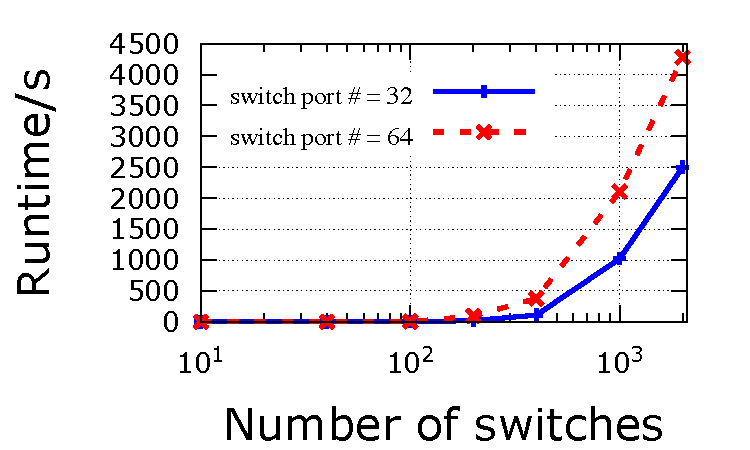
\includegraphics[width=0.3\textwidth] {figs/algo_runtime}
	\caption{Runtime of Algorithm~\ref{alg:greedy} for Jellyfish network of different sizes.}
	\label{fig:algo_runtime}
	\vspace{-0.25in}
\end{figure}

\subsection{Impact on throughout and latency}\label{subsec:exp_performanceoverhead}

\begin{figure}[t]
	\centering
	
	\subfloat[short for lof][Throughput] {
		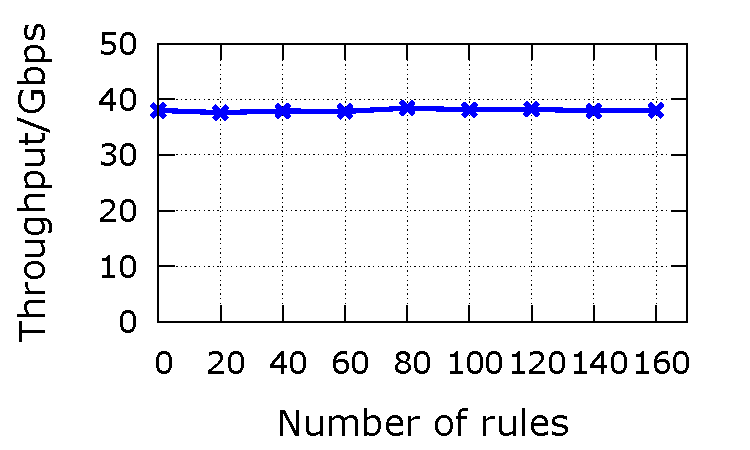
\includegraphics[width=0.25\textwidth] {figs/overhead_avgthrpt}
	}
	\subfloat[short for lof][Latency]{
		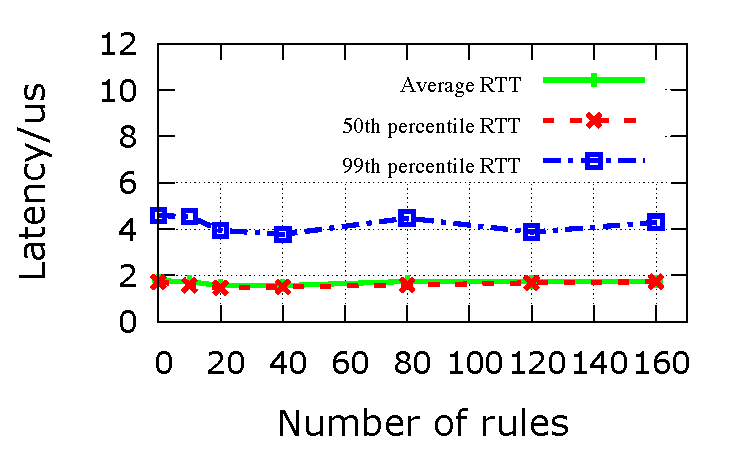
\includegraphics[width=0.25\textwidth] {figs/RDMAlatency_overhead}
	}
	
		\caption{\sysname{} has no impact on throughput and latency}
		\label{fig:perf_penalty}
\end{figure}

On datapath, packets have to traverse the rules installed by \sysname{}.  These
rules installed in TCAM, and hence have no discernible impact on throughput and
latency. We installed different number of \sysname{} rules on T1, and measured
average throughput and latency between H1 and H2 over several runs.
Figure~\ref{fig:perf_penalty} confirms that throughput and latency are not
affected by the number of rules.


%\subsection{Simple demonstration of \sysname{}}\label{subsec:exp_demon}
%	
%	\begin{figure}[t]
%		%\vspace{-0.1in}
%		\centering
%		
%		\subfloat[short for lof][Experiment scenario.]{
%			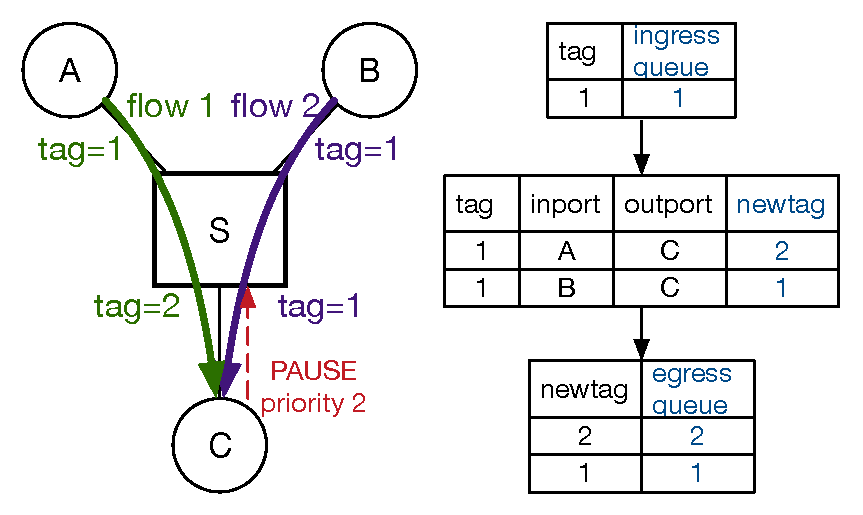
\includegraphics[width=0.25\textwidth] {figs/demon_scenario}
%		}
%		\subfloat[short for lof][Rate of flow 1 and flow 2.]{
%			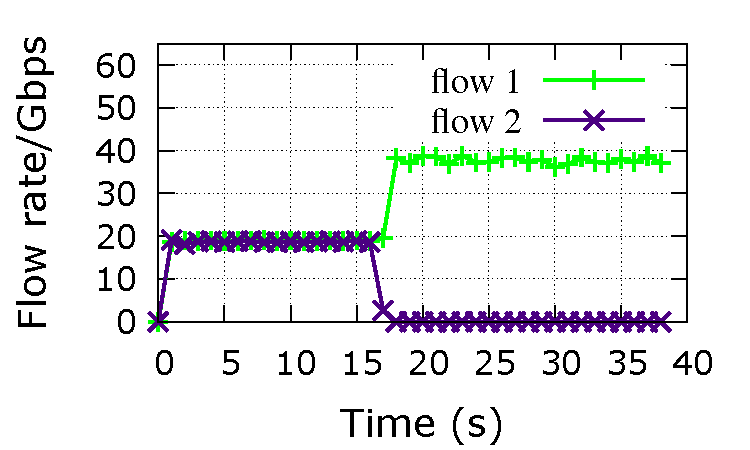
\includegraphics[width=0.25\textwidth] {figs/demon_flowrate}
%		}
%		
%		\caption{The match-action rules in action}\label{fig:tagger_demon}
%	\end{figure}
%	
%	
%A simple experiment shown in
%Figure~\ref{fig:tagger_demon} demonstrates the behavior of the match-action
%rules.  We generate two flows, flow 1 and flow 2, to send packets to C from
%different servers connected to ports A and B. Both servers set the DSCP value in
%outgoing packets to 1. The match-action rules are set to rewrite the tag value
%of packets arriving on port A to 2, and forward them to port C. Tag of packets
%arriving on port B is not changed.
%
%At time = 17s, C sends a stream of forged PFC PAUSE frames on priority 2 to
%switch S. The rate of both flows is plotted in Figure~\ref{fig:tagger_demon}(b)
%(link capacity = 40Gbps). As expected, after priority 2 is paused, rate of
%flow 1 is reduced to 0 while flow 2 gets all the available bandwidth.
%Counters on switch S further confirm that no packets were dropped, and server
%connected to port A was paused as expected.
